%%%%% Set up %%%%%

% Set document style and font size
\documentclass[12pt]{article}\usepackage[]{graphicx}\usepackage[]{color}
%% maxwidth is the original width if it is less than linewidth
%% otherwise use linewidth (to make sure the graphics do not exceed the margin)
\makeatletter
\def\maxwidth{ %
  \ifdim\Gin@nat@width>\linewidth
    \linewidth
  \else
    \Gin@nat@width
  \fi
}
\makeatother

\definecolor{fgcolor}{rgb}{0.345, 0.345, 0.345}
\newcommand{\hlnum}[1]{\textcolor[rgb]{0.686,0.059,0.569}{#1}}%
\newcommand{\hlstr}[1]{\textcolor[rgb]{0.192,0.494,0.8}{#1}}%
\newcommand{\hlcom}[1]{\textcolor[rgb]{0.678,0.584,0.686}{\textit{#1}}}%
\newcommand{\hlopt}[1]{\textcolor[rgb]{0,0,0}{#1}}%
\newcommand{\hlstd}[1]{\textcolor[rgb]{0.345,0.345,0.345}{#1}}%
\newcommand{\hlkwa}[1]{\textcolor[rgb]{0.161,0.373,0.58}{\textbf{#1}}}%
\newcommand{\hlkwb}[1]{\textcolor[rgb]{0.69,0.353,0.396}{#1}}%
\newcommand{\hlkwc}[1]{\textcolor[rgb]{0.333,0.667,0.333}{#1}}%
\newcommand{\hlkwd}[1]{\textcolor[rgb]{0.737,0.353,0.396}{\textbf{#1}}}%
\let\hlipl\hlkwb

\usepackage{framed}
\makeatletter
\newenvironment{kframe}{%
 \def\at@end@of@kframe{}%
 \ifinner\ifhmode%
  \def\at@end@of@kframe{\end{minipage}}%
  \begin{minipage}{\columnwidth}%
 \fi\fi%
 \def\FrameCommand##1{\hskip\@totalleftmargin \hskip-\fboxsep
 \colorbox{shadecolor}{##1}\hskip-\fboxsep
     % There is no \\@totalrightmargin, so:
     \hskip-\linewidth \hskip-\@totalleftmargin \hskip\columnwidth}%
 \MakeFramed {\advance\hsize-\width
   \@totalleftmargin\z@ \linewidth\hsize
   \@setminipage}}%
 {\par\unskip\endMakeFramed%
 \at@end@of@kframe}
\makeatother

\definecolor{shadecolor}{rgb}{.97, .97, .97}
\definecolor{messagecolor}{rgb}{0, 0, 0}
\definecolor{warningcolor}{rgb}{1, 0, 1}
\definecolor{errorcolor}{rgb}{1, 0, 0}
\newenvironment{knitrout}{}{} % an empty environment to be redefined in TeX

\usepackage{alltt}

% File path to resources (style file etc)
\newcommand{\locRepo}{csas-style}

% Style file for DFO Technical Reports
\usepackage{\locRepo/tech-report}

% header-includes from R markdown entry
\usepackage{pdflscape}

%%%%% Variables %%%%%

% New definitions: Title, year, report number, authors
% Protect lower case words (i.e., species names) in \Addlcwords{}, in "TechReport.sty"
\newcommand{\trTitle}{Estimation of fork length using cranial measurements of sablefish (\emph{Anoplopoma fimbria}).}
\newcommand{\trYear}{2021}
\newcommand{\trReportNum}{nnn}
% Optional
\newcommand{\trAuthFootA}{Email: \href{mailto:Kathryn.Temple@dfo-mpo.gc.ca}{\nolinkurl{Kathryn.Temple@dfo-mpo.gc.ca}} \textbar{} telephone: (250) 756-7366}
\newcommand{\trAuthsLong}{Kathryn x. Temple and Kendra Holt and Lisa C. Lacko}
\newcommand{\trAuthsBack}{Kathryn x. Temple, K. Holt and Lacko, L.C.}

% New definition: Address
\newcommand{\trAddy}{Pacific Biological Station\\
Fisheries and Oceans Canada, 3190 Hammond Bay Road\\
Nanaimo, British Columbia, V9T 6N7, Canada\\}

% Abstract
\newcommand{\trAbstract}{Routine biological sampling of whole round sablefish from commercial fishing operations have occurred since the early 1990's. Historically, specimens have been obtained through a voluntary catch sampling program and tagged sablefish recovery program. In order to improve the quantity and size range of samples received, we investigated the potential for obtaining biological information using heads, rather than the entire fish. In 2016, 438 sablefish (240-1080 mm) were sampled at sea and six different fish head measurements were assessed to see if they could predict fork length. Genetic samples (100) were collected to develop methods for DNA-based sex identification. A pilot study was conducted in 2017 with head-only samples and sex determination provided by a commercial vessel, followed by scientific sampling on shore. Regression analysis results show that the interorbital distance measurement was a good predictor of sablefish fork length, while samplers ranked it the most efficient and easily repeatable. Genetic results indicate xx\% accuracy in fisher sex detection. Subsequently, the 2018 sampling collection program was modified so that returns of whole round sablefish were replaced by head-only samples with knife cuts on the operculum to indicate sex.}

% Resume (i.e., French abstract)
\newcommand{\trResume}{}

\newcommand{\trISBN}{}

%%%%% Start %%%%%

% Start the document
\IfFileExists{upquote.sty}{\usepackage{upquote}}{}
\begin{document}

%%%% Front matter %%%%%

% Add the first few pages
\frontmatter

%%%%% Drafts %%%%%

%\linenumbers  % Line numbers
%\onehalfspacing  % Extra space between lines
\renewcommand{\headrulewidth}{0.5pt}  % Header line
\renewcommand{\footrulewidth}{0.5pt}  % footer line
%\pagestyle{fancy}\fancyhead[c]{Draft: Do not cite or circulate}  % Header text

%%%%% Main document %%%%%
\hypertarget{introduction}{%
\section{Introduction}\label{introduction}}

Biological samples of British Columbia (BC) sablefish (\emph{Anoplopoma fimbria}) have been collected from commercial fishing operations since 1995 (Haist and Wyeth \protect\hyperlink{ref-Haist2001}{2001}) and processed by the Department of Fisheries and Oceans (DFO) port samplers and contracted service providers. In addition, tagged fish recovered in commercial fisheries (trap, trawl, hook and line) have been received at the point of landing via the dockside monitoring program (DMP) and sampled by Archipelago Marine Research (AMR) since the early 1990's. These data provide a fishery dependent source of age composition data for the two-sex structured operating model of the coastal Management Strategy Evaluation (MSE) (Cox et al. \protect\hyperlink{ref-Cox2019}{2019}).

Movement to a head only catch sampling program was initiated to improve the number of returns and increase the range of sizes in the samples. Six fish head dimension measurements of upper jaw length, eye diameter, interorbital distance, snout length, post orbital to preoperculum distance and post orbital head length were obtained from the 212 sablefish caught during the 2016 West Coast Vancouver Island (WCVI) survey (Williams et al. \protect\hyperlink{ref-Williams2018}{2018}) and 219 sablefish caught during the 2016 West Coast Haida Gwaii (WCHG) survey (Nottingham et al. \protect\hyperlink{ref-Nottingham2018}{2018}). Seven small sablefish were collected during the 201? salmon survey (Figure~\ref{fig:figure1}).

Regression models were developed by using measurements taken from 216 females and 222 males sampled in 2016.

\hypertarget{methods}{%
\section{Methods}\label{methods}}

\#\#Estimation of Fork Length using Cranial Measurements

Mitutoyo ABSOLUTE® 500-762-20 Coolant Proof Digimatic Caliper

\hypertarget{survey-sample-collection}{%
\subsubsection{Survey sample collection}\label{survey-sample-collection}}

Measurements of fork length (FL), round weight (RW), upper jaw length (UJ), eye diameter (ED), interorbital distance (IO), snout length (SL), post orbital to preoperculum distance (PP), and post orbital head length (PH) were obtained from sablefish caught on selected surveys (Table~\ref{tab:table1}). Fish sex and maturity were recorded and sagittal otoliths and operculum clips (DNA) were collected at sea.

\hypertarget{pilot-study-sample-collection}{%
\subsubsection{Pilot study sample Collection}\label{pilot-study-sample-collection}}

In 2017, a pilot study was conducted with the commercial sector returning sablefish heads, rather than the entire fish. A total of 360 heads were collected from J-cut sablefish on a trip to the S\(\text{\underline{G}}\)aan \(\text{\underline{K}}\)inghlas - Bowie (SK-B) seamount. Each operculum was marked with either one knife cut (male) or two knife cuts (female) (Appendix~\ref{app:second-appendix} ). The first 99 heads of the pilot study were measured by three technicians for IO, SN, UJ and PP lengths.

\hypertarget{sampling-on-shore}{%
\subsubsection{Sampling on shore}\label{sampling-on-shore}}

On shore, the heads were thawed, and cranial dimensions were measured using electronic calipers. Ageing structures (sagittal otoliths) were also collected from each head. Operculum clips were collected from the first 137 fish measured (79 male and 58 female), and were stored in vials containing 95\% ethanol, to be used for DNA extraction and the development of a genetic test for fish gender.

\hypertarget{head-measurements}{%
\subsubsection{Head measurements}\label{head-measurements}}

The six cranial dimensions were ranked by samplers on a five point rating scale in terms of ease of use and repeatability with electronic Mitutoyo 500 series calipers. The ease of use metric focused on three key attributes of measurement learnability (task understanding), efficiency (task-completion time) and difficulty (task performance ease). The repeatability metric focused on ranking the efficiency of a measurement for repeated caliper placement, taking into consideration the soft and hard head tissues.

\hypertarget{genetic-test-development}{%
\subsection{Genetic test development}\label{genetic-test-development}}

DNA multiplex polymerase chain reactions (PCRs) were conducted using fluorescently labelled forward primers. X-insert and Y-insert specific primers developed by Rondeau et al. (\protect\hyperlink{ref-Rondeau2013}{2013}) were used, but the X-insert forward and Y-nested reverse were redesigned to produce slightly smaller PCR products.

\hypertarget{pilot-study}{%
\subsection{Pilot study}\label{pilot-study}}

\hypertarget{discussion}{%
\section{Discussion}\label{discussion}}

Routine biological sampling procedures have been modified so that commercial fisheries are now only returning heads, rather than entire fish.

\clearpage

\hypertarget{results}{%
\section{Results}\label{results}}

\hypertarget{sample-collection}{%
\section{Sample collection}\label{sample-collection}}

The endemic and endangered status makes, P. denisonii an important freshwater species of study and the biometrics information is useful for more effective management of in-situ conservation. A total of 306 specimens comprising 111 males, 97 females and 98 indeterminate were used for the study. The smallest length of captured fish was 3.30 cm and highest was 14.00 cm in TL (Table 1).

A total of 438 specimens comprising xx males and xx females were collected for six head measurements (UJ,ED,IO,SL, PP, PH), fork length, round weight, otoliths and DNA. Post orbital head length (Posterior inner edge of orbit to dorsal insertion of opercle) was also measured, but this was abandoned after 130 measurements, to save time, and because it was not possible to measure this on a number of the heads for a variety of reasons (opercula had been cut off from some heads, it was awkward to take longer measurements using the electronic calipers, and the end points of the measurement were difficult to define.

The mean values of the predictor and response variables (Table~\ref{tab:table2}).

Given the ease of measurement, we suggest that Interorbital distance be used to predict sablefish fork lengths and weights (Table~\ref{tab:table3}).

We found evidence of relationships between upper jaw length and fork length (p = \ensuremath{9.358\times 10^{-278}}) ; eye diameter and fork length (p = \ensuremath{5.34\times 10^{-203}}); interorbital distance and fork length (p = \ensuremath{5.539\times 10^{-272}} ); upper snout length and fork length (p = \ensuremath{4.593\times 10^{-292}}); postorbital to preoperculum length and fork length (p = \ensuremath{2.024\times 10^{-247}}); and postorbital head length and fork length (p = 0).

The estimated slope is 7.695 (SE 0.088) units of fork length per unit of upper jaw length; the estimated slope is 21.994 (SE 0.389) units of fork length per unit of eye diameter; the estimated slope is 11.622 (SE 0.138) units of fork length per unit of interorbital distance; the estimated slope is 11.182 (SE 0.118 units of fork length per unit of snout length; the estimated slope is 14.373 (SE 0.191) units of fork length per unit of postorbital to preoperculum length; and the estimated slope is 6.83 (SE 0.185) units of fork length per unit of postorbital head length.

\hypertarget{pilot-collection-of-sablefish-heads-as-a-biological-sample}{%
\section{Pilot Collection of Sablefish Heads as a Biological Sample}\label{pilot-collection-of-sablefish-heads-as-a-biological-sample}}

Heads were received by DFO in good condition (intact and not deformed), segregated by set, for measuring and otolith extraction. Operculum cuts worked well to indicate sex

\hypertarget{repeatability-of-measurements-between-technicians}{%
\section{Repeatability of measurements between technicians}\label{repeatability-of-measurements-between-technicians}}

\clearpage

\hypertarget{tables}{%
\section{Tables}\label{tables}}



\begin{table}[!h]

\caption{\label{tab:table1}Description of head dimensions measured and description of caliper jaw positions. ~\\
\hspace*{0.333em}\\}
\fontsize{10}{12}\selectfont
\begin{tabular}[t]{>{\raggedright\arraybackslash}p{1.9cm}>{\raggedright\arraybackslash}p{6.0cm}>{\raggedright\arraybackslash}p{7.5cm}}
\toprule
\textbf{Head dimension} & \textbf{Head description} & \textbf{Caliper jaw position}\\
\midrule
UJ & Tip of snout to the posterior edge of the maxilla. & Outside caliper jaw measurement from forward point and centre of snout to back of maxilla.\\
\midrule
ED & Anterior-posterior diameter of eye socket. & Inside caliper jaw measurement firmly stretched against eye socket at vertical midpoint of eye.\\
\midrule
IO & Narrowest distance between eye sockets, measured on dorsal surface. & Outside caliper jaw measurement of the horizontal midpoint of eyes on dorsal surface.\\
\midrule
SL & Tip of snout to anterior inner edge of eye socket. & Outside caliper jaw measurement from forward point and centre of snout to horizontal midpoint of anterior edge of eye socket.\\
\midrule
PP & Posterior inner edge of orbit to visual insertion point of preopercle. & Outside caliper jaw measurement from back of eye socket to preopercle bone insertion point. Preopercle must be lifted to expose preopercle bone underneath.\\
\midrule
\addlinespace
PH & Posterior inner edge of orbit to dorsal insertion of opercle. & Outside caliper jaw measurement from back of eye socket to bone underneath gill cover notch at dorsal insertion of the opercle.  The operculum must be held taut.\\
\bottomrule
\end{tabular}
\end{table}
~\\
\hspace*{0.333em}\\


\begin{table}[!h]

\caption{\label{tab:table2}Summary of sablefish biological data collected. Tally of fork lengths (FL), round weight (RW), upper jaw length (UJ), eye diameter (ED), interorbital distance (IO), snout length (SL), post orbital to preoperculum distance (PP), post orbital head length (PH), females (F), males (M), sagittal otoliths (O) and operculum clips (DNA) listed by survey. ~\\
\hspace*{0.333em}\\}
\fontsize{10}{12}\selectfont
\begin{tabular}[t]{lrrrrrrrrrrrrr}
\toprule
\textbf{Survey} & \textbf{FL} & \textbf{RW} & \textbf{UJ} & \textbf{ED} & \textbf{IO} & \textbf{SL} & \textbf{PP} & \textbf{PH} & \textbf{F} & \textbf{M} & \textbf{Otoliths} & \textbf{DNA} & \textbf{Total}\\
\midrule
2016 WCHG & 219 & 219 & 219 & 219 & 218 & 219 & 207 & 52 & 111 & 108 & 219 & 59 & 219\\
2016 WCVI & 212 & 212 & 211 & 212 & 212 & 211 & 212 & 78 & 105 & 107 & 212 & 78 & 212\\
Salmon & 7 & 0 & 7 & 7 & 7 & 7 & 7 & 0 & 0 & 7 & 0 & 0 & 7\\
\bottomrule
\end{tabular}
\end{table}

\begin{table}[!h]

\caption{\label{tab:table3}Table of sample size, mean and standard deviation for predictor and response variables for each head dimension. ~\\}
\fontsize{10}{12}\selectfont
\begin{tabular}[t]{>{\raggedright\arraybackslash}p{4.9cm}>{\raggedright\arraybackslash}p{0.6cm}>{\raggedright\arraybackslash}p{0.6cm}>{\raggedright\arraybackslash}p{1.6cm}>{\raggedright\arraybackslash}p{2.1cm}>{\raggedright\arraybackslash}p{0.8cm}>{\raggedright\arraybackslash}p{0.6cm}}
\toprule
\textbf{Predictor variable} & \textbf{n} & \textbf{mean} & \textbf{sd} & \textbf{Response variable} & \textbf{mean} & \textbf{sd}\\
\midrule
Upper jaw length & 437 & 57.95 & 15.22 & Fork length & 573.27 & 120.44\\
Eye diameter & 438 & 25.9 & 5.13 & Fork length & 573.3 & 120.3\\
InterOrbital distance & 437 & 40.37 & 10.06 & Fork length & 573.36 & 120.43\\
Snout length & 437 & 44.81 & 10.52 & Fork length & 573.27 & 120.44\\
Post orbital to preoperculum length & 426 & 31.5 & 8.02 & Fork length & 571.34 & 119.54\\
Post orbital head length & 130 & 60.85 & 18.87 & Fork length & 566.46 & 134.8\\
\bottomrule
\end{tabular}
\end{table}


on each head dimension manual calipers for \textgreater15cm distances other metrics indicate if calipers were limited after \textgreater15 cm, bilateral measurements were possible and if the measurement involved bone.
\begin{table}

\caption{\label{tab:table4}Ease of use and repeatability considerations for each measurement.number, ease of use and repeatability five point ranking where 5-Great; 4- Good; 3-Moderate; 2-Questionable; 1-Terrible.}
\fontsize{10}{12}\selectfont
\begin{tabular}[t]{>{\raggedright\arraybackslash}p{1.0cm}>{\raggedleft\arraybackslash}p{0.6cm}>{\raggedleft\arraybackslash}p{1.7cm}>{\raggedright\arraybackslash}p{1.2cm}>{\raggedright\arraybackslash}p{1.7cm}>{\raggedright\arraybackslash}p{1.7cm}>{\raggedright\arraybackslash}p{4.2cm}}
\toprule
\multicolumn{1}{c}{\textbf{ }} & \multicolumn{2}{c}{\textbf{5 Point}} & \multicolumn{1}{c}{\textbf{ }} & \multicolumn{2}{c}{\textbf{Measurement}} & \multicolumn{1}{c}{\textbf{ }} \\
\cmidrule(l{3pt}r{3pt}){2-3} \cmidrule(l{3pt}r{3pt}){5-6}
Head Dimension & Ease of use & Repeatable & Caliper limitation & Bilateral measurement & Bone measurement & Considerations\\
\midrule
UJ & 3 & 4 & x & x & x & End of the maxilla difficult to define. Caliper jaw position must be in center of snout.\\
\midrule
ED & 3 & 2 &  & x &  & Caliper outside jaw position on soft tissue in eye socket may result in measurement differences.\\
\midrule
IO & 5 & 5 &  &  & x & Tissue is compressed to obtain bone measurement. Easy to determine caliper jaw position.\\
\midrule
SL & 4 & 5 &  & x & x & Caliper jaw position must be in center of snout.\\
\midrule
PP & 4 & 5 &  & x & x & Caliper position on pre-operculum may result in measurement differences.\\
\midrule
PH & 3 & 2 & x & x &  & Operculum damage from handling was observed on several fish.\\
\bottomrule
\end{tabular}
\end{table}

\begin{table}

\caption{\label{tab:table5}Estimated slope and}
\fontsize{10}{12}\selectfont
\begin{tabular}[t]{lll}
\toprule
\textbf{Head dimension} & \textbf{slope} & \textbf{SE}\\
\midrule
Upper jaw length & 7.6946 & 0.088\\
Eye diameter & 21.994 & 0.389\\
InterOrbital distance & 11.622 & 0.138\\
Snout length & 11.182 & 0.118\\
Post orbital to preoperculum length & 14.373 & 0.191\\
Post orbital head length & 6.8299 & 0.185\\
\bottomrule
\end{tabular}
\end{table}
\clearpage

\hypertarget{figures}{%
\section{Figures}\label{figures}}


\begin{figure}[htb]

{\centering \pdftooltip{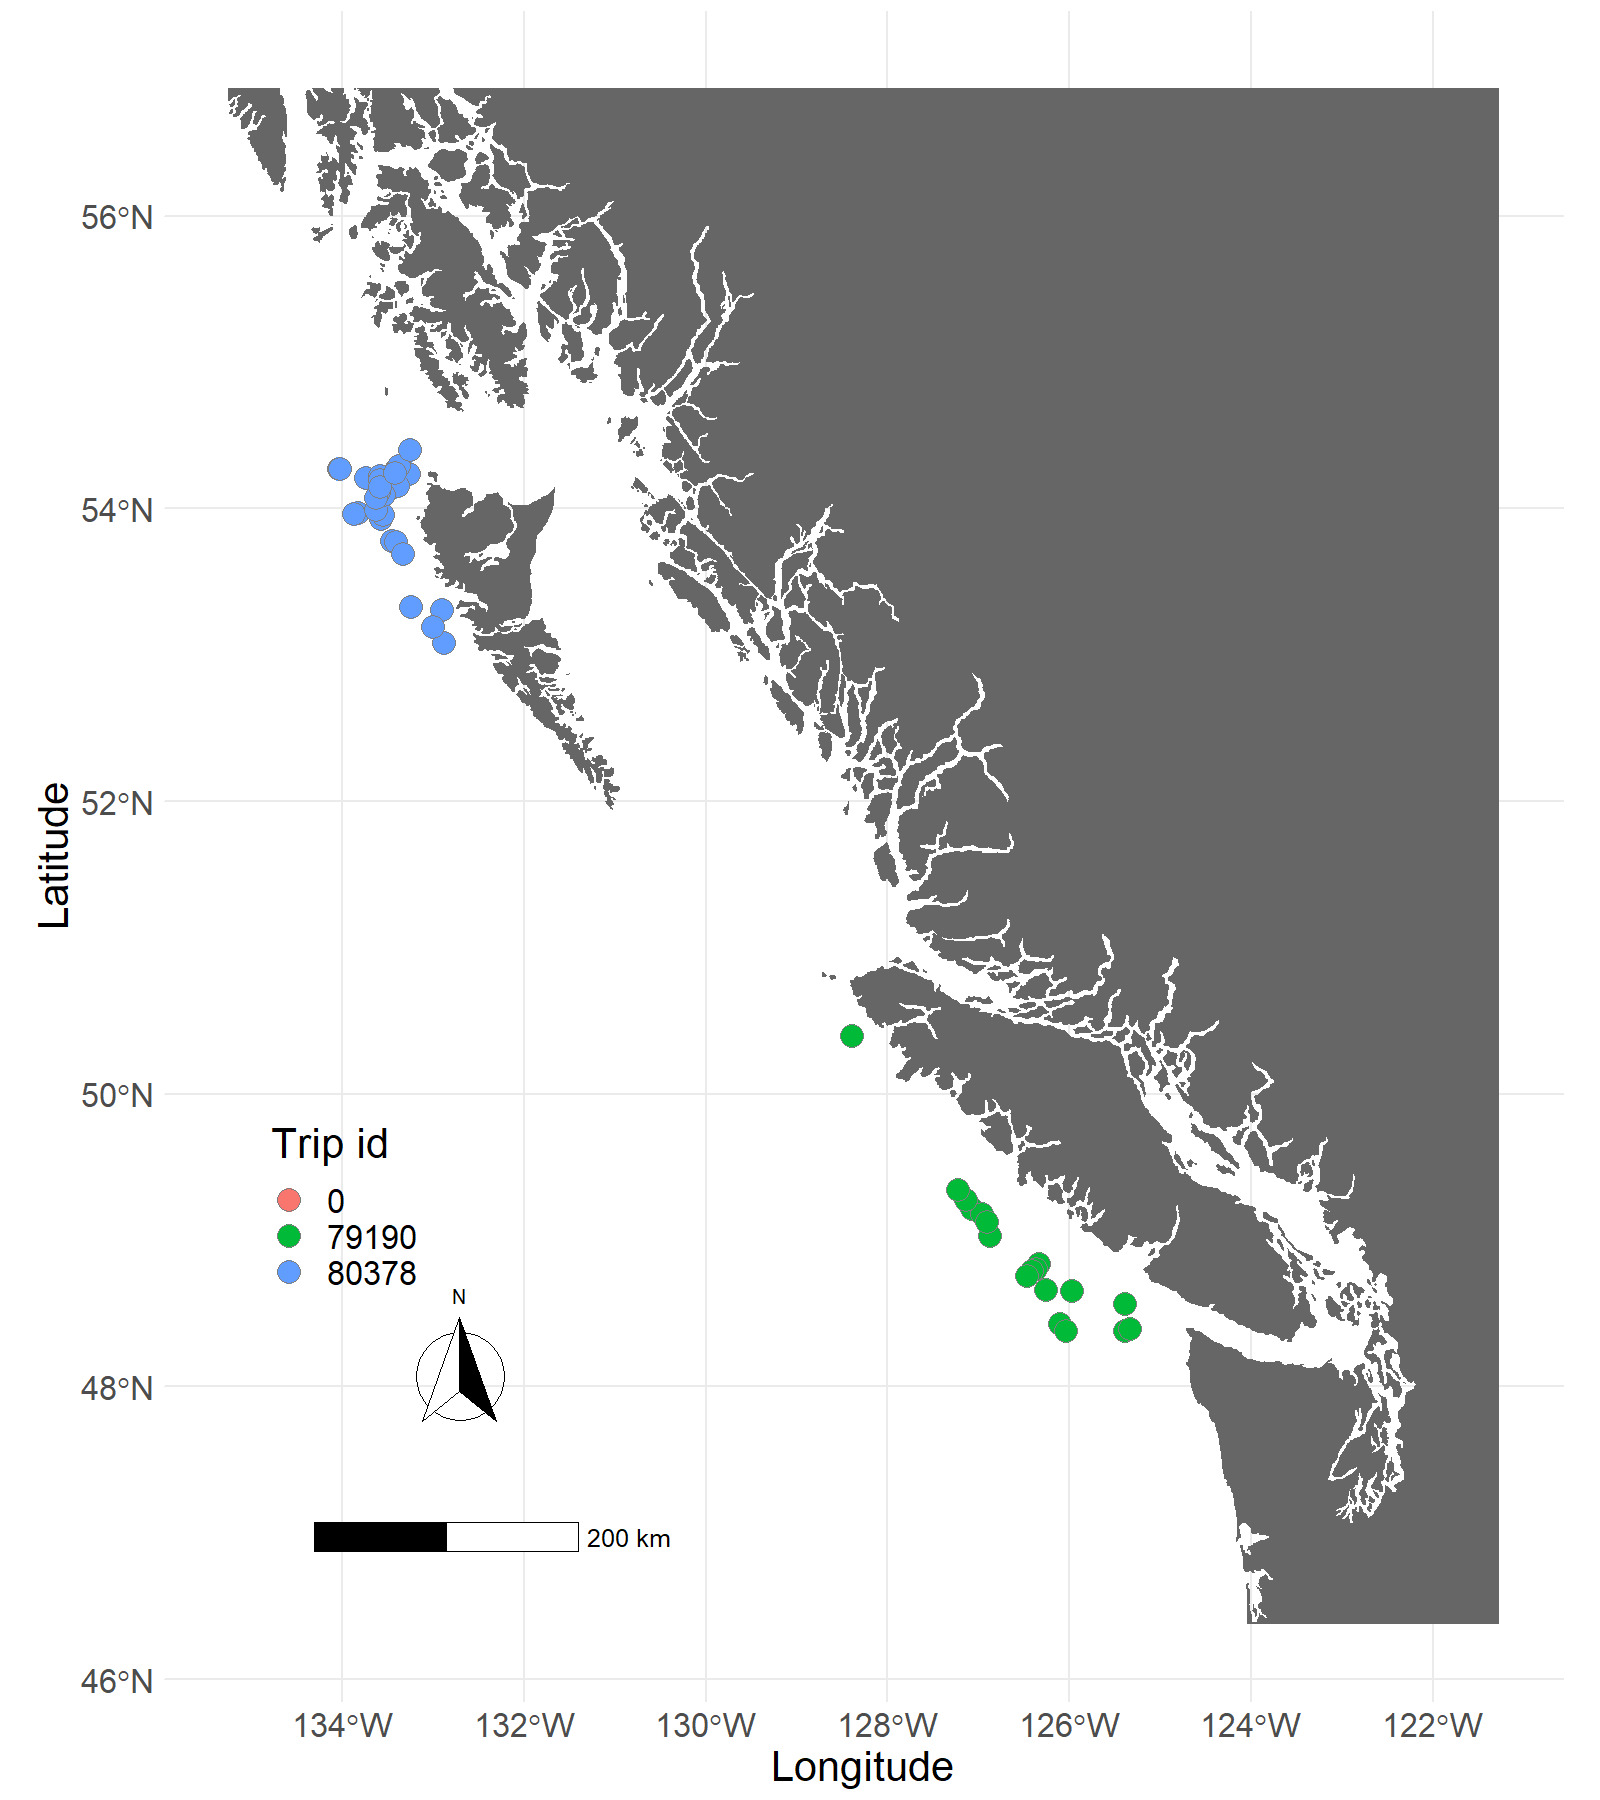
\includegraphics[width=6in]{C:/github/sablehead/figures/Figure1}}{Figure \ref{fig:figure1}} 

}

\caption{Sample locations in 2016 from the WCVI survey (GFBIO trip id 79190), WCHG survey (GFBIO trip id 80378) and salmon survey (?).}\label{fig:figure1}
\end{figure}

\begin{figure}[htb]

{\centering \pdftooltip{\includegraphics[width=400px,height=290px]{C:/github/sablehead/figures/figure2}}{Figure \ref{fig:figure2}} 

}

\caption{Scatterplot upper jaw vs fork length, measurements in millimeters.}\label{fig:figure2}
\end{figure}

\begin{figure}[htb]

{\centering \pdftooltip{\includegraphics[width=400px,height=290px]{C:/github/sablehead/figures/figure3}}{Figure \ref{fig:figure3}} 

}

\caption{Scatterplot eye diameter vs fork length, measurements in millimeters.}\label{fig:figure3}
\end{figure}

\begin{figure}[htb]

{\centering \pdftooltip{\includegraphics[width=400px,height=290px]{C:/github/sablehead/figures/figure4}}{Figure \ref{fig:figure4}} 

}

\caption{Scatterplot interorbital vs fork length.}\label{fig:figure4}
\end{figure}

\begin{figure}[htb]

{\centering \pdftooltip{\includegraphics[width=400px,height=290px]{C:/github/sablehead/figures/figure5}}{Figure \ref{fig:figure5}} 

}

\caption{Scatterplot snout length vs fork length.}\label{fig:figure5}
\end{figure}

\begin{figure}[htb]

{\centering \pdftooltip{\includegraphics[width=400px,height=290px]{C:/github/sablehead/figures/figure6}}{Figure \ref{fig:figure6}} 

}

\caption{Scatterplot post orbital to preoperculum length vs fork length.}\label{fig:figure6}
\end{figure}

\begin{figure}[htb]

{\centering \pdftooltip{\includegraphics[width=400px,height=290px]{C:/github/sablehead/figures/figure7}}{Figure \ref{fig:figure7}} 

}

\caption{Scatterplot of post orbital length vs fork length.}\label{fig:figure7}
\end{figure}
\clearpage

\hypertarget{discussion-1}{%
\section{Discussion}\label{discussion-1}}

Interorbial head length (IO) proved to be a good predictor of fork length for sablefish.

\hypertarget{acknowledgments}{%
\section{Acknowledgments}\label{acknowledgments}}

We thank \ldots{}

\begin{appendices}
\counterwithin{figure}{section}
\counterwithin{table}{section}
\counterwithin{equation}{section}

\clearpage

\section{IMAGES OF THE SIX CRANIAL DIMENSION MEASUREMENTS.}
\label{app:first-appendix}

A. Upper jaw measurement (UJ); B. Eye diameter measurement (ED); C. Interorbital distance (ID); D. Snout length (SL); E. Post orbital to preoperculum length measurement (PP); F. Post orbital head length (PH).
\begin{center}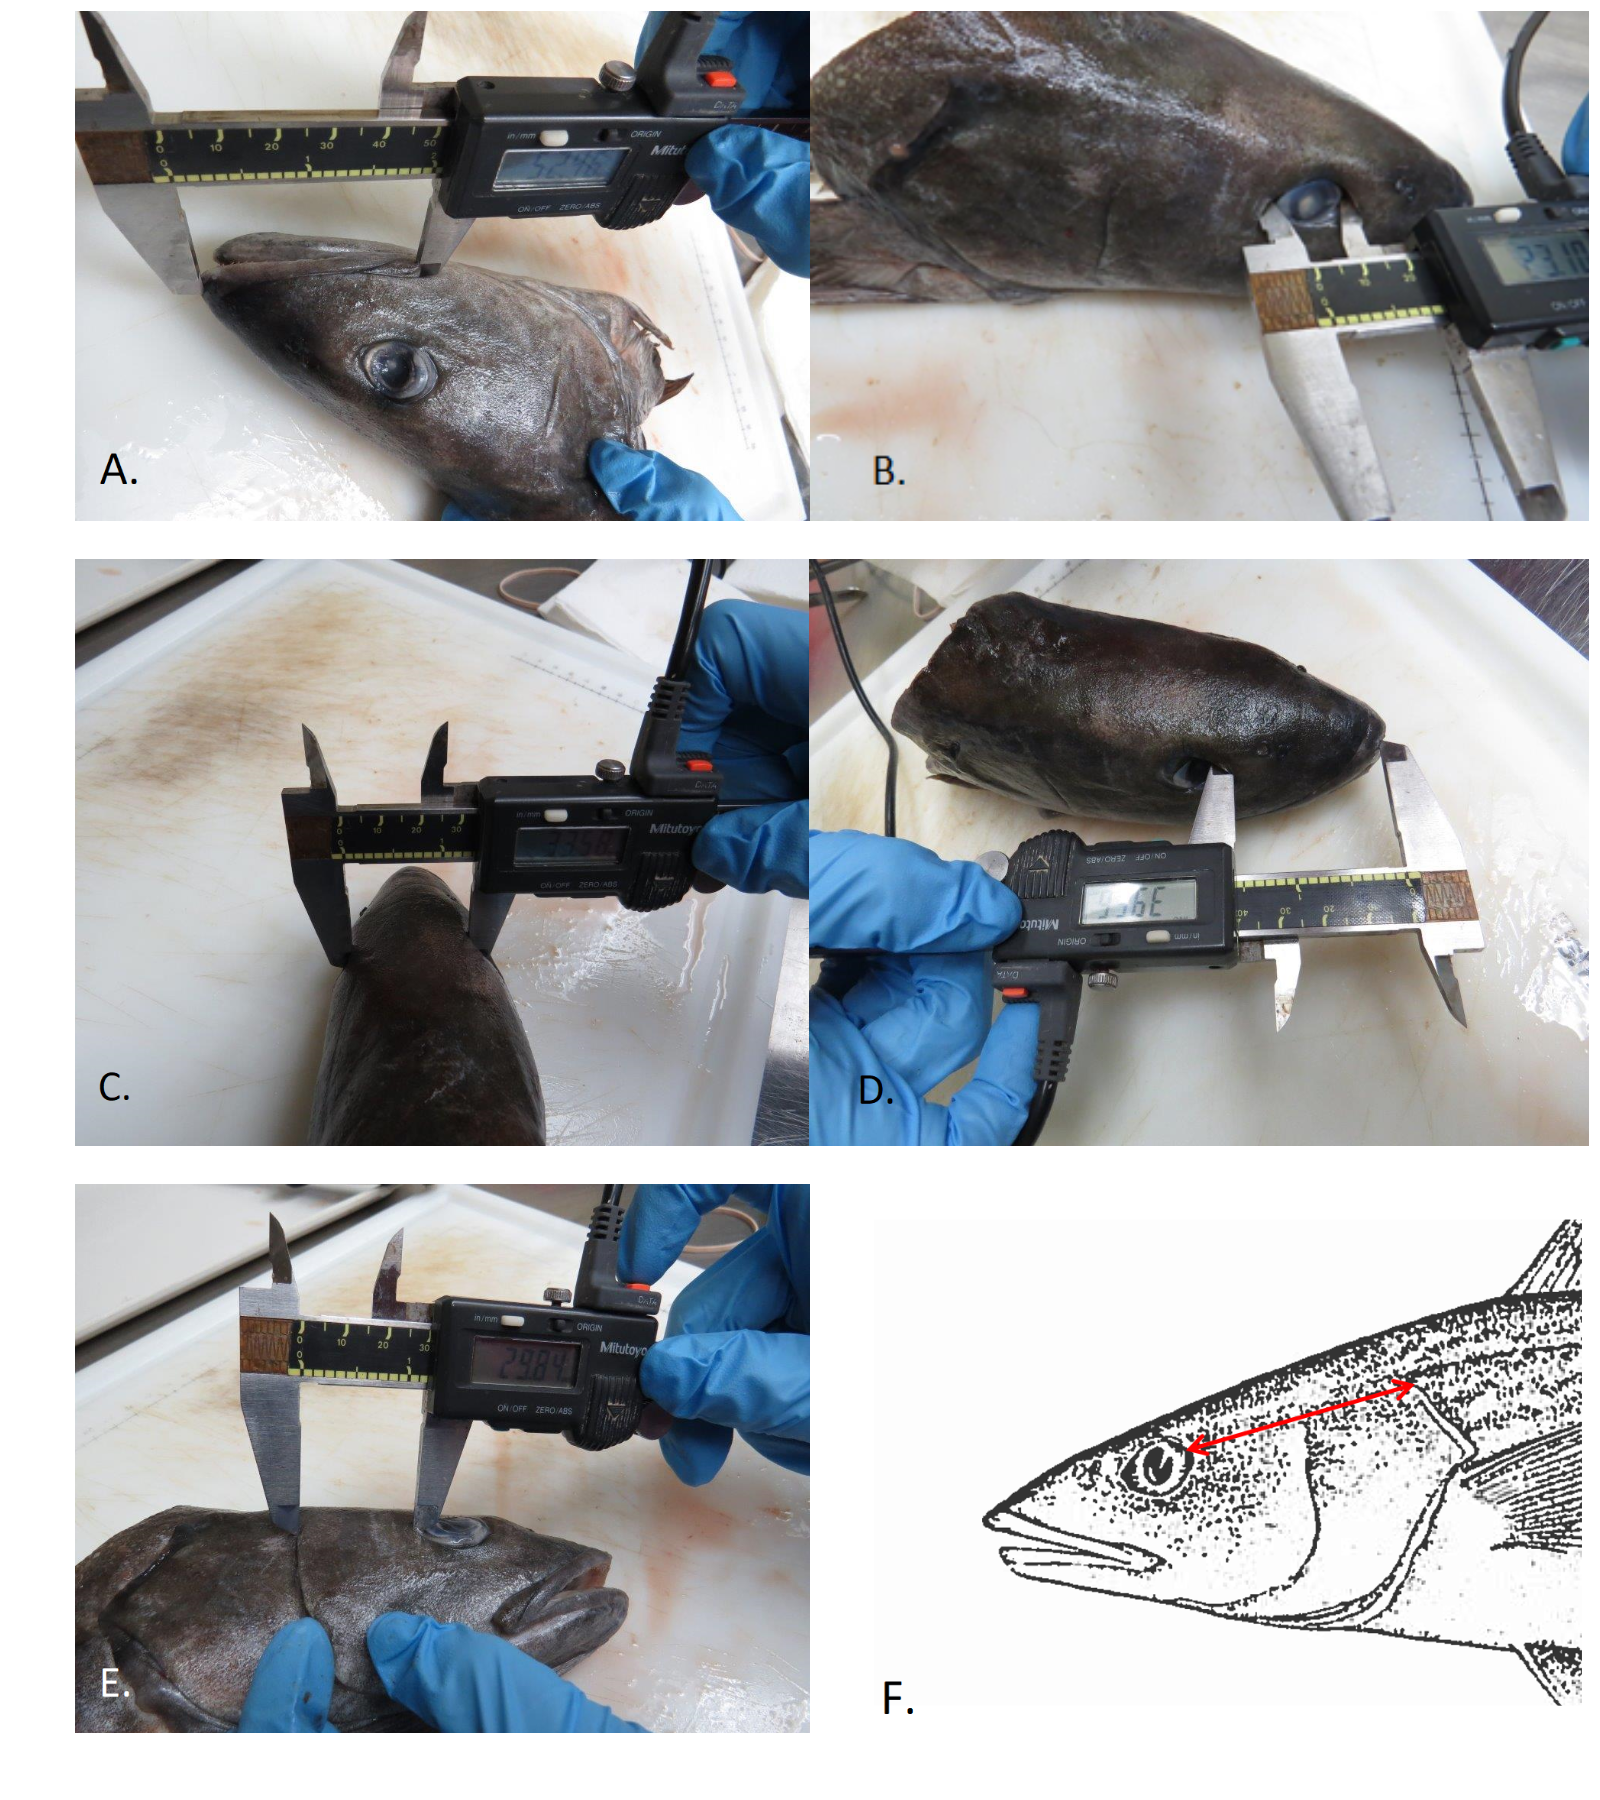
\includegraphics[width=6in]{C:/github/sablehead/figures/AppendixA} \end{center}

\clearpage

\section{SEX DETERMINATION BY OPERCULUM MARKING}
\label{app:second-appendix}

Operculum knife cuts for sablefish males (A) and females (B).
\begin{center}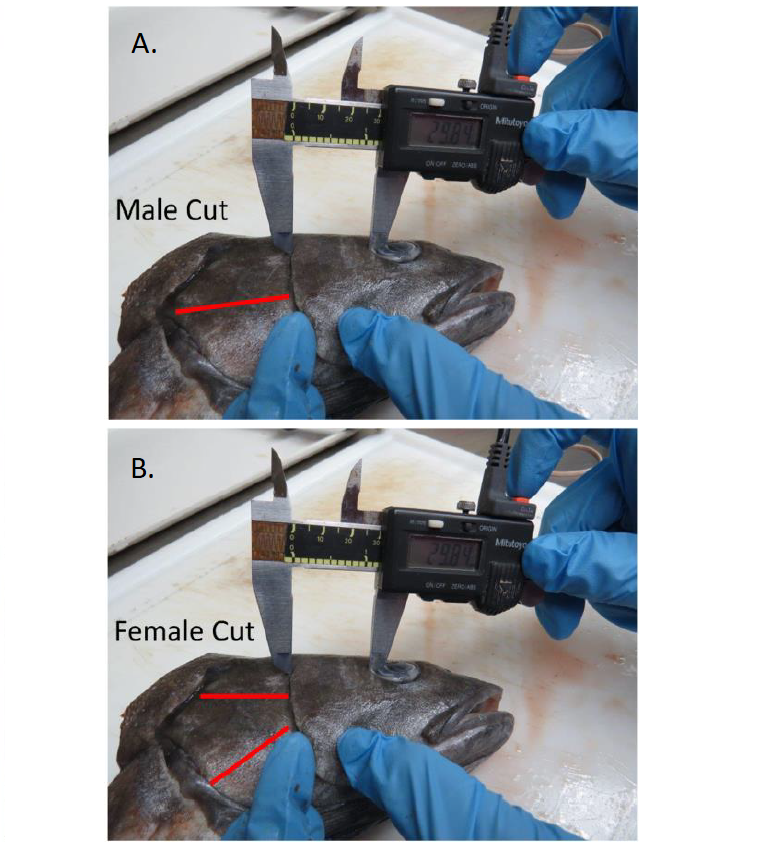
\includegraphics[width=6in]{C:/github/sablehead/figures/AppendixB} \end{center}
\clearpage

\end{appendices}

\hypertarget{refs}{}
\leavevmode\hypertarget{ref-Cox2019}{}%
Cox, S.P., Holt, K., and Johnson, S. 2019. Evaluating the robustness of management procedures for the Sablefish (*anoplopoma fimbria*) fishery in British Columbia, Canada for 2017-18. DFO Can. Sci. Advis. Sec. Res. Doc. 2019/032: vi + 79 p.

\leavevmode\hypertarget{ref-Haist2001}{}%
Haist, R.H., V., and Wyeth, M. 2001. Sablefish Stock Assessment for 2001 and Advice to Managers for 2002. DFO Can. Sci. Advis. Sec. Res. Doc. 2001/135.

\leavevmode\hypertarget{ref-Nottingham2018}{}%
Nottingham, M.K., Williams, D.C., Wyeth, M.R., and Olsen, N. 2018. Summary of the west coast haida gwaii synoptic bottom trawl survey, august 25 - september 26, 2016. Can. Manuscr. Rep. Fish. Aquat. Sci. 3151: viii: 51 p.

\leavevmode\hypertarget{ref-Rondeau2013}{}%
Rondeau, E.B., Messmer, A.M., Sanderson, D.S., Jantzen, S.G., Schalburg, K.R. von, Minkley, D.R., Leong, J.S., Macdonald, G.M., Davidsen, A.E., Parker, W.A., Mazzola, R.S.A., Campbell, B., and Koop, B.F. 2013. Genomics of sablefish (anoplopoma fimbria): Expressed genes, mitochondrial phylogeny, linkage map and identification of a putative sex gene. BMC Genomics 14(1): 452. Journal Article.

\leavevmode\hypertarget{ref-Williams2018}{}%
Williams, D.C., Nottingham, M.K., Olsen, N., and Wyeth, M.R. 2018. Summary of the west coast vancouver island synoptic bottom trawl survey, may 24 - june 15, 2016. Can. Manuscr. Rep. Fish. Aquat. Sci. 3137: viii: 54 p.
\end{document}
